\documentclass{article}
% Some basic packagesLLuu
\usepackage[utf8]{inputenc}
\usepackage{spverbatim}
\usepackage[margin=1.2in]{geometry}
\usepackage{textcomp}
\usepackage{url}
\usepackage{graphicx}
\usepackage{float}
\usepackage{enumitem}
\usepackage{standalone}
\usepackage{tcolorbox}
\usepackage{wrapfig}
% \usepackage{svg}
% \usepackage{svg-inkscape} 

\graphicspath{{./figures}}

%color settings
\usepackage{xcolor}
\definecolor{gruvbgdark}{HTML}{1d2021}
\definecolor{gruvtextdark}{HTML}{ebdbb2}
\definecolor{gruvbglight}{HTML}{f9f5d7}
\definecolor{gruvtextlight}{HTML}{3c3836}
\definecolor{NavyBlue}{HTML}{266bbd}
\definecolor{RawSienna}{HTML}{94330e}
\definecolor{ForestGreen}{HTML}{149b52}
% \pagecolor{gruvbgdark}
% \color{gruvtextdark}

% Hide page number when page is empty
\usepackage{emptypage}
\usepackage{subcaption}
\usepackage{multicol}

% Math stuff
\usepackage{amsmath, amsfonts, mathtools, amsthm, amssymb}
% Fancy script capitals
\usepackage{mathrsfs}
\usepackage{cancel}

% Bold math
\usepackage{bm}

% SVG setup
% \svgsetup{inkscapeexe=inkscape, inkscapearea=drawing}
% \svgpath{~/dev/DAVE3700-Matte-3000/figures/}

% Some shortcuts
\newcommand\N{\ensuremath{\mathbb{N}}}
\newcommand\R{\ensuremath{\mathbb{R}}}
\newcommand\Z{\ensuremath{\mathbb{Z}}}
\renewcommand\O{\ensuremath{\emptyset}}
\newcommand\Q{\ensuremath{\mathbb{Q}}}
\newcommand\C{\ensuremath{\mathbb{C}}}

%Make implies and impliedby shorter
\let\implies\Rightarrow
\let\impliedby\Leftarrow
\let\iff\Leftrightarrow

\let\epsilon\varepsilon

% Add \contra symbol to denote contradiction
% \usepackage{stmaryrd} % for \lightning
% \newcommand\contra{\scalebox{1.5}{$\lightning$}}

\let\phi\varphi

% Command for short corrections
% Usage: 1+1=\correct{3}{2}

\definecolor{correct}{HTML}{009900}
\newcommand\correct[2]{\ensuremath{\:}{\color{red}{#1}}\ensuremath{\to }{\color{correct}{#2}}\ensuremath{\:}}
\newcommand\green[1]{{\color{correct}{#1}}}

% horizontal rule
% \newcommand\hr{
%     \noindent\rule[0.5ex]{\linewidth}{0.5pt}
% }

% hide parts
\newcommand\hide[1]{}

% Environments
\makeatother

% For box around Definition, Theorem, \ldots
% theorems
\usepackage{thmtools}
\usepackage[framemethod=TikZ]{mdframed}
\mdfsetup{skipabove=1em,skipbelow=1em, innertopmargin=5pt, innerbottommargin=6pt}

\theoremstyle{definition}

\makeatletter

% \declaretheoremstyle[headfont=\bfseries, bodyfont=\normalfont, mdframed={ nobreak } ]{thmgreenbox}
% \declaretheoremstyle[headfont=\bfseries, bodyfont=\normalfont, mdframed={ nobreak } ]{thmredbox}
% \declaretheoremstyle[headfont=\bfseries, bodyfont=\normalfont, spaceabove=0.5cm, spacebelow=0.5cm]{thmbluebox}
% % \declaretheoremstyle[headfont=\bfseries, bodyfont=\normalfont]{thmbluebox}
% \declaretheoremstyle[headfont=\bfseries, bodyfont=\normalfont]{thmblueline}
% \declaretheoremstyle[headfont=\bfseries, bodyfont=\normalfont, numbered=no, mdframed={ rightline=false, topline=false, bottomline=false, }, qed=\qedsymbol ]{thmproofbox}
% \declaretheoremstyle[headfont=\bfseries\sffamily, bodyfont=\normalfont, numbered=no, mdframed={ nobreak, rightline=false, topline=false, bottomline=false } ]{thmexplanationbox}
\declaretheoremstyle[headfont=\bfseries, bodyfont=\normalfont, numbered=no]{idea}

\declaretheoremstyle[
	headfont=\bfseries\color{ForestGreen!70!black}, bodyfont=\normalfont,
	mdframed={
			linewidth=2pt,
			rightline=false, topline=false, bottomline=false,
			linecolor=ForestGreen, backgroundcolor=ForestGreen!5,
		}
]{thmgreenbox}

\declaretheoremstyle[
	headfont=\bfseries\color{NavyBlue!70!black}, bodyfont=\normalfont,
	mdframed={
			linewidth=2pt,
			rightline=false, topline=false, bottomline=false,
			linecolor=NavyBlue, backgroundcolor=NavyBlue!5,
		}
]{thmbluebox}

\declaretheoremstyle[
	headfont=\bfseries\color{NavyBlue!70!black}, bodyfont=\normalfont,
	mdframed={
			linewidth=2pt,
			rightline=false, topline=false, bottomline=false,
			linecolor=NavyBlue
		}
]{thmblueline}

\declaretheoremstyle[
	headfont=\bfseries\color{RawSienna!70!black}, bodyfont=\normalfont,
	mdframed={
			linewidth=2pt,
			rightline=false, topline=false, bottomline=false,
			linecolor=RawSienna, backgroundcolor=RawSienna!5,
		}
]{thmredbox}

\declaretheoremstyle[
	headfont=\bfseries\color{RawSienna!70!black}, bodyfont=\normalfont,
	numbered=no,
	mdframed={
			linewidth=2pt,
			rightline=false, topline=false, bottomline=false,
			linecolor=RawSienna, backgroundcolor=RawSienna!5,
		},
	qed=\qedsymbol
]{thmproofbox}

\declaretheoremstyle[
	headfont=\bfseries\color{NavyBlue!70!black}, bodyfont=\normalfont,
	numbered=no,
	mdframed={
			linewidth=2pt,
			rightline=false, topline=false, bottomline=false,
			linecolor=NavyBlue, backgroundcolor=NavyBlue!1,
		},
]{thmexplanationbox}

\declaretheorem[style=thmgreenbox, name=Definisjon]{definition}
\declaretheorem[sibling=definition, style=thmredbox, name=Corollary]{corollary}
\declaretheorem[style=thmbluebox, numbered=no, name=Idea]{idea}
\declaretheorem[style=idea, style=thmredbox, name=Proposition]{prop}
\declaretheorem[sibling=definition, style=thmredbox, name=Theorem]{theorem}
\declaretheorem[sibling=definition, style=thmredbox, name=Lemma]{lemma}



\declaretheorem[numbered=no, style=thmexplanationbox, name=Proof]{explanation}
\declaretheorem[numbered=no, style=thmproofbox, name=Bevis]{replacementproof}
\declaretheorem[style=thmgreenbox,  numbered=no, name=Oppgave]{ex}
\declaretheorem[style=thmbluebox,  numbered=no, name=Eksempel]{eg} \declaretheorem[style=thmblueline, numbered=no, name=Remark]{remark}
\declaretheorem[style=thmblueline, numbered=no, name=Merk]{note}

\renewenvironment{proof}[1][\proofname]{\begin{replacementproof}}{\end{replacementproof}}

\AtEndEnvironment{eg}{\null\hfill$\diamond$}%

\newtheorem*{uovt}{UOVT}
\newtheorem*{notation}{Notation}
\newtheorem*{previouslyseen}{As previously seen}
\newtheorem*{problem}{Problem}
\newtheorem*{observe}{Observe}
\newtheorem*{property}{Property}
\newtheorem*{intuition}{Intuition}


% Exercise 
% Usage:
% \oefening{5}
% \suboefening{1}
% \suboefening{2}
% \suboefening{3}
% gives
% Oefening 5
%   Oefening 5.1
%   Oefening 5.2
%   Oefening 5.3
\newcommand{\oefening}[1]{%
	\def\@oefening{#1}%
	\subsection*{Oefening #1}
}

\newcommand{\suboefening}[1]{%
	\subsubsection*{Oefening \@oefening.#1}
}


% \lecture starts a new lecture (les in dutch)
%
% Usage:
% \lecture{1}{di 12 feb 2019 16:00}{Inleiding}
%
% This adds a section heading with the number / title of the lecture and a
% margin paragraph with the date.

% I use \dateparts here to hide the year (2019). This way, I can easily parse
% the date of each lecture unambiguously while still having a human-friendly
% short format printed to the pdf.

% \usepackage{xifthen}
% \def\testdateparts#1{\dateparts#1\relax}
% \def\dateparts#1 #2 #3 #4 #5\relax{
% 	\marginpar{\small\textsf{\mbox{#1 #2 #3 #5}}}
% }

% \def\@lecture{}%
% \newcommand{\lecture}[3]{
% 	\ifthenelse{\isempty{#3}}{%
% 		\def\@lecture{Lecture #1}%
% 	}{%
% 		\def\@lecture{Lecture #1: #3}%
% 	}%
% 	\subsection*{\@lecture}
% 	% \marginpar{\small\textsf{\mbox{#2}}}
% }

\usepackage{listings}

\definecolor{dkgreen}{rgb}{0,0.6,0}
\definecolor{gray}{rgb}{0.5,0.5,0.5}
\definecolor{mauve}{rgb}{0.58,0,0.82}

\lstset{frame=none,
  language=Haskell,
  aboveskip=3mm,
  belowskip=3mm,
  showstringspaces=false,
  columns=flexible,
  basicstyle={\small\ttfamily},
  numbers=none,
  numberstyle=\tiny\color{gray},
  keywordstyle=\color{blue},
  commentstyle=\color{dkgreen},
  stringstyle=\color{mauve},
  breaklines=true,
  breakatwhitespace=true,
  tabsize=3
}



% These are the fancy headers
\usepackage{fancyhdr}
\pagestyle{fancy}

% LE: left even
% RO: right odd
% CE, CO: center even, center odd
% My name for when I print my lecture notes to use for an open book exam.
\fancyhead[LE,RO]{Kristian Sørdal}

\fancyhead[RO,LE]{INF122 - Funksjonell Programmering} % Right odd,  Left even
% \fancyhead[RE,LO]{\leftmark}          % Right even, Left odd
\fancyhead[RE,LO]{Kristian Sørdal}          % Right even, Left odd

\fancyfoot[RO,LE]{\thepage}  % Right odd,  Left even
% \fancyfoot[RE,LO]{Kristian Sørdal}          % Right even, Left odd
\fancyfoot[C]{\leftmark}     % Center

\makeatother

% Todonotes and inline notes in fancy boxes
\usepackage{todonotes}
\usepackage{tcolorbox}

% Make boxes breakable
\tcbuselibrary{breakable}

% Figure support as explained in my blog post.
\usepackage{import}
\usepackage{xifthen}
\usepackage{pdfpages}
\usepackage{transparent}
\newcommand{\incfig}[2][1]{%
	% \begin{center}
	\def\svgwidth{#1\columnwidth}
	\import{./figures/}{#2.pdf_tex}
	% \end{center}
}
% Fix some stuff
% %http://tex.stackexchange.com/questions/76273/multiple-pdfs-with-page-group-included-in-a-single-page-warning
\pdfsuppresswarningpagegroup=1
\author{Kristian Sørdal}


\begin{document}
    \section{Forelesning 3}

    \subsubsection{Plan for forelesningen}

    Vi begynner på lista fra forrige gang:

    \begin{itemize}
        \item Tuppler
        \item Maybe
        \item Lister
        \item Either
        \item Map
    \end{itemize}

    Vi kommer definitivt ikke lenger enn til lister idag.

    \subsection{Tuppler: Eksempeltyper}

    Tuppeltyper skrives med paranteser og komma:

    \begin{itemize}
        \item \texttt{(Integer, String)} er typen av alle par av heltall og strenger.
        \item \texttt{(Double,Double,Double)} er typen av alle 3D koordinater, eller vektorer, med dobbel presisjonsflyttall.
    \end{itemize}
    \begin{align*}
        & \vdots \\
        &\text{osv}
    \end{align*}

    \subsubsection{Sammenligning med lister}

    \begin{itemize}
        \item Tuppler: Fiksert antall posisjoner for data.
        \item Hver posisjon har en type.
        \item Lister: Variabelt antall posisjoner for data (lengde)
        \item Lister: Alle elementer i listen har samme type.
    \end{itemize}

\subsubsection{Kanonsike verdier}

De kanoniske verdiene i tuppeltypene er de på formen:

\subsubsection{Funksjoner definert med møn}

\begin{eg}
    La oss skrive en funksjon som normaliserer en vektor. (Det vil si å skalere den slik at den har lengde 1.)

    \begin{figure}[H]
        \begin{center}
            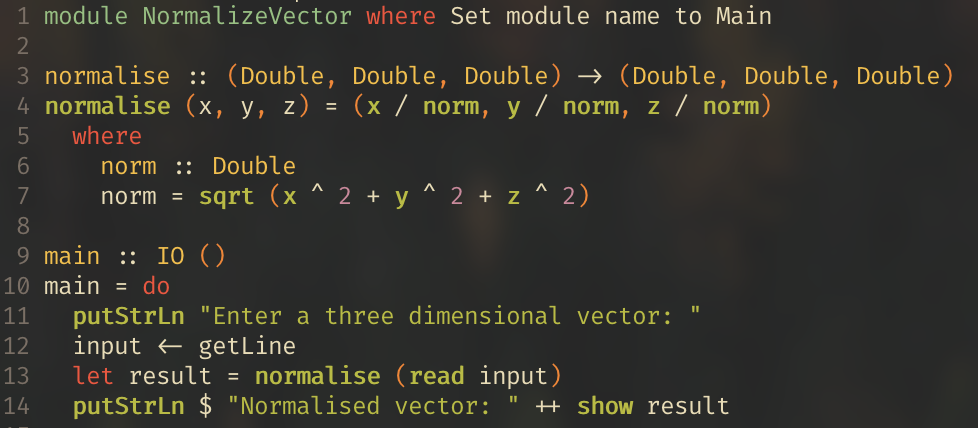
\includegraphics[width=0.95\textwidth]{normvec.png}
        \end{center}
    \end{figure}
\end{eg}

Generelt definerer vi mønster matching hvordan funksjonen opererer på en kanonisk verdi av typen.
\medskip

\( \left( 1,2,3 \right) \) er en kanonisk verdi av typen \texttt{(Double, Double, Double)}

\subsubsection{Projeksjoner}
For par (tupler med to posisjoner), har vi to funksjoner for å hente ut data fra et par:

\begin{align*}
    &\texttt{fst :: (a, b) -> a} \\
\end{align*}

\subsection{Currying}
En funksjon som tar to verdier har vi sett kan ha type på formen:

\[ \texttt{A -> B -> C} \]

Eksempel fra boken

\begin{align*}
    &\texttt{add :: (Integer, Integer) -> Integer} \\ 
    &\texttt{add (x, y) = x + y}\\
    &\texttt{add' :: Integer -> Integer -> Integer}\\
    &\texttt{add' x y = x + y}
\end{align*}

\subsubsection{Fordeler med begge}
Fordelen med currying er partiell applikasjon

\[ \texttt{add' 3 :: Integer -> Integer} \]

Fordelen med uncurrying er at det er lett å mappe funksjonen inn i en struktur:

\[ > map add 3 [(1,2), (2,1), (0,3)] \]

\subsubsection{Funksjoner for å gå frem og tilbake}

Gjøre en funksjon curried:

\[ \texttt{curry :: ((a,b) -> c) -> a -> b -> c} \]

Gjøre en funksjon uncurried:

\[ \texttt{uncurry :: (a -> b -> c) -> (a,b) -> c} \]

\subsubsection{Hva er konvensjonen i Haskell}

Standard i Haskell er å definere funksjonen som ferdig curry-et, og heller bruke uncurry eksplisitt der det er behov.

\[ \texttt{map (uncurry (+)) [(x,y) | x <- [0..3], y <- [x..3]]} \]

\subsection{Maybe}

Vi lager \textit{Maybe-typer} ved å skrive \texttt{Maybe} foran typen

\begin{itemize}
    \item \texttt{Maybe Integer} er typen av kanskje heltall
\end{itemize}

\begin{eg}
    Eksempler på elementer

    \begin{align*}
        &\texttt{Just 3 :: Maybe Integer} \\
        &\texttt{Nothing :: Maybe Integer}
    \end{align*}

    \[ \texttt{readMaybe :: String -> Maybe Integer} \]

    \begin{note}
        \texttt{readMaybe} må importeres fra \texttt{Text.Read}
    \end{note}
\end{eg}

\subsubsection{Konstruktører}

Maybe typene har to konstruktører
\begin{itemize}
    \item \texttt{Nothing :: Maybe a}
    \item \texttt{Just :: a -> Maybe a}
\end{itemize}

\subsubsection{Nyttige funksjoner}

La oss se på noen nyttige funksjoner

\begin{itemize}
    \item \texttt{maybe :: b -> (a -> b) -> Maybe a -> b}
    \item \texttt{fromMaybe :: a -> Maybe a -> a}
    \item \texttt{fmap :: (a -> b) -> Maybe a -> Maybe b}
\end{itemize}

Man kan også få ut boolske verdier fra en Maybe-verdi

\subsection{Lister}

\begin{itemize}
    \item \texttt{[Integer]} er en liste av heltall
    \item \texttt{[Char] = String} er en streng / liste med characters 
    \item \texttt{[[Integer]]} er en liste med lister av heltall
    \item \texttt{[Double -> Double]} er en liste med funksjoner på flyttal
\end{itemize}

\subsubsection{Konstruktører}

Lister har to konstruktører

\begin{itemize}
    \item \texttt{[] :: [a]} - Den tomme listen
    \item \texttt{(:) :: a -> [a] -> [a]} - Legger et element foran i listen
\end{itemize}

Dermed er kanoniske element i en listetype \texttt{[A]} de som er på formen

\begin{itemize}
    \item \texttt{[]} eller
    \item \texttt{a : as} hvor \texttt{a :: A} og \texttt{as :: [A]}
\end{itemize}

Syntaktisk sukker \texttt{[1,2,3,]} istedetfor \texttt{1:2:3:[]}

\subsubsection{Mønster}

Vi kan definere funksjoner på lister ved hjelp av mønster som matcher \texttt{(:)} og \texttt{[]:}

\begin{align*}
    &\texttt{safeHead :: [a] -> Maybe a} \\
    &\texttt{safeHead}
\end{align*}

\subsubsection{Rekursjon}

Senere skal vi se hvordan vi kan definere alle mulige funksjoner på lister vha. rekusjon

\begin{align*}
    &\texttt{duplicate :: [a] -> [a]} \\
    &\texttt{dublicate [] = []} \\
    &\texttt{duplicate (a : as) = a : a : duplicate as}
\end{align*}
\end{document}
